\documentclass{article}
% translate with >> pdflatex -shell-escape <file>

% This file is an extract of the PGFPLOTS manual, copyright by Christian Feuersaenger.
% 
% Feel free to use it as long as you cite the pgfplots manual properly.
%
% See
%   http://pgfplots.sourceforge.net/pgfplots.pdf
% for the complete manual.
%
% Any required input files (for <plot table> or <plot file> or the table package) can be downloaded
% at
% http://www.ctan.org/tex-archive/graphics/pgf/contrib/pgfplots/doc/latex/
% and
% http://www.ctan.org/tex-archive/graphics/pgf/contrib/pgfplots/doc/latex/plotdata/

\usepackage{pgfplots}
\pgfplotsset{compat=newest}

\pagestyle{empty}
\usepackage{nicefrac}

\begin{document}
% \usepackage{nicefrace}% required
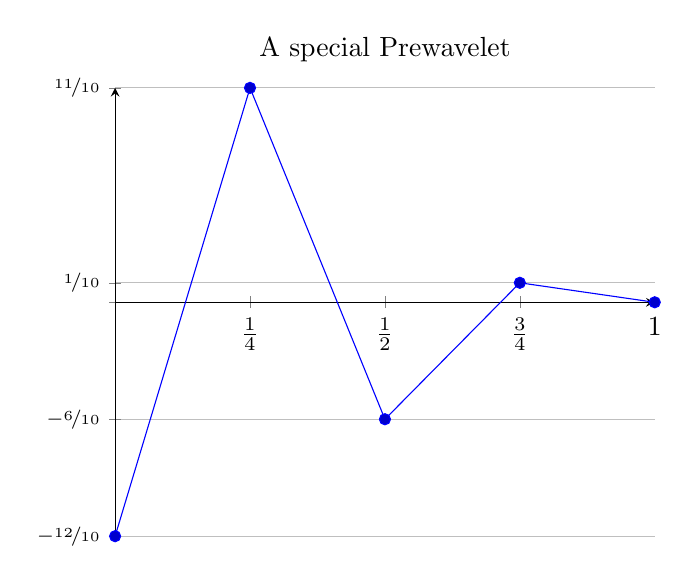
\begin{tikzpicture}
\begin{axis}[
	% x ticks explicitly formatted:
	xtick={0,1,0.5,0.25,0.75},
	xticklabels={$0$,$1$,$\frac12$,$\frac14$,$\frac34$},
	% y ticks automatically by some code fragment:
	ytick=data,
	yticklabel={%
		\scriptsize
		\ifdim\tick pt<0pt % a TeX \if -- see TeX Book
			\pgfmathparse{-10*\tick}%
			$-\nicefrac{\pgfmathprintnumber{\pgfmathresult}}{10}$%
		\else
			\ifdim\tick pt=0pt
			\else
				\pgfmathparse{10*\tick}%
				$\nicefrac{\pgfmathprintnumber{\pgfmathresult}}{10}$%
			\fi
		\fi
	},
	% NOTE: this here does the same:
	% yticklabel style={/pgf/number format/.cd,frac,
	% 	frac TeX=\nicefrac,frac whole=false,frac denom=10},
	ymajorgrids,
	title=A special Prewavelet,
	axis x line=center,
	axis y line=left,
	]
	\addplot coordinates {(0,-1.2) (0.25,1.1) 
		(0.5,-0.6) (0.75,0.1) (1,0)};
\end{axis}
\end{tikzpicture}
\end{document}
